% Options for packages loaded elsewhere
\PassOptionsToPackage{unicode}{hyperref}
\PassOptionsToPackage{hyphens}{url}
%
\documentclass[
]{article}
\usepackage{amsmath,amssymb}
\usepackage{lmodern}
\usepackage{ifxetex,ifluatex}
\ifnum 0\ifxetex 1\fi\ifluatex 1\fi=0 % if pdftex
  \usepackage[T1]{fontenc}
  \usepackage[utf8]{inputenc}
  \usepackage{textcomp} % provide euro and other symbols
\else % if luatex or xetex
  \usepackage{unicode-math}
  \defaultfontfeatures{Scale=MatchLowercase}
  \defaultfontfeatures[\rmfamily]{Ligatures=TeX,Scale=1}
\fi
% Use upquote if available, for straight quotes in verbatim environments
\IfFileExists{upquote.sty}{\usepackage{upquote}}{}
\IfFileExists{microtype.sty}{% use microtype if available
  \usepackage[]{microtype}
  \UseMicrotypeSet[protrusion]{basicmath} % disable protrusion for tt fonts
}{}
\makeatletter
\@ifundefined{KOMAClassName}{% if non-KOMA class
  \IfFileExists{parskip.sty}{%
    \usepackage{parskip}
  }{% else
    \setlength{\parindent}{0pt}
    \setlength{\parskip}{6pt plus 2pt minus 1pt}}
}{% if KOMA class
  \KOMAoptions{parskip=half}}
\makeatother
\usepackage{xcolor}
\IfFileExists{xurl.sty}{\usepackage{xurl}}{} % add URL line breaks if available
\IfFileExists{bookmark.sty}{\usepackage{bookmark}}{\usepackage{hyperref}}
\hypersetup{
  pdftitle={Digital Literacy Predicts Accuracy Judgments in Misinformation},
  hidelinks,
  pdfcreator={LaTeX via pandoc}}
\urlstyle{same} % disable monospaced font for URLs
\usepackage[margin=1in]{geometry}
\usepackage{longtable,booktabs,array}
\usepackage{calc} % for calculating minipage widths
% Correct order of tables after \paragraph or \subparagraph
\usepackage{etoolbox}
\makeatletter
\patchcmd\longtable{\par}{\if@noskipsec\mbox{}\fi\par}{}{}
\makeatother
% Allow footnotes in longtable head/foot
\IfFileExists{footnotehyper.sty}{\usepackage{footnotehyper}}{\usepackage{footnote}}
\makesavenoteenv{longtable}
\usepackage{graphicx}
\makeatletter
\def\maxwidth{\ifdim\Gin@nat@width>\linewidth\linewidth\else\Gin@nat@width\fi}
\def\maxheight{\ifdim\Gin@nat@height>\textheight\textheight\else\Gin@nat@height\fi}
\makeatother
% Scale images if necessary, so that they will not overflow the page
% margins by default, and it is still possible to overwrite the defaults
% using explicit options in \includegraphics[width, height, ...]{}
\setkeys{Gin}{width=\maxwidth,height=\maxheight,keepaspectratio}
% Set default figure placement to htbp
\makeatletter
\def\fps@figure{htbp}
\makeatother
\setlength{\emergencystretch}{3em} % prevent overfull lines
\providecommand{\tightlist}{%
  \setlength{\itemsep}{0pt}\setlength{\parskip}{0pt}}
\setcounter{secnumdepth}{5}
\ifluatex
  \usepackage{selnolig}  % disable illegal ligatures
\fi
\newlength{\cslhangindent}
\setlength{\cslhangindent}{1.5em}
\newlength{\csllabelwidth}
\setlength{\csllabelwidth}{3em}
\newenvironment{CSLReferences}[2] % #1 hanging-ident, #2 entry spacing
 {% don't indent paragraphs
  \setlength{\parindent}{0pt}
  % turn on hanging indent if param 1 is 1
  \ifodd #1 \everypar{\setlength{\hangindent}{\cslhangindent}}\ignorespaces\fi
  % set entry spacing
  \ifnum #2 > 0
  \setlength{\parskip}{#2\baselineskip}
  \fi
 }%
 {}
\usepackage{calc}
\newcommand{\CSLBlock}[1]{#1\hfill\break}
\newcommand{\CSLLeftMargin}[1]{\parbox[t]{\csllabelwidth}{#1}}
\newcommand{\CSLRightInline}[1]{\parbox[t]{\linewidth - \csllabelwidth}{#1}\break}
\newcommand{\CSLIndent}[1]{\hspace{\cslhangindent}#1}

\title{Digital Literacy Predicts Accuracy Judgments in Misinformation}
\author{Dan Xu\\
University of Toronto}
\date{2022-02-14}

\begin{document}
\maketitle
\begin{abstract}
This project is a replication for ``\href{https://misinforeview.hks.harvard.edu/article/digital-literacy-is-associated-with-more-discerning-accuracy-judgments-but-not-sharing-intentions/}{Digital literacy is associated with more discerning accuracy judgments but not sharing intentions}.'' Through two survey experiments with a sample of 1,341 U.S. respondents, Sirlin et al. (2021) find that digital literacy is positively associated with misinformation discernment, but not with sharing intention. I performed Ordinary Least-squares regression analyses to replicate their research, and my results show consistency with their findings. In addition, the results show that age is negatively associated with digital literacy.
\end{abstract}

\hypertarget{introduction}{%
\section{Introduction}\label{introduction}}

Misinformation has been exacerbating the public trust in political and societal institutions. It is widely assumed that a lack of digital literacy - an individual's ability to fluently use digital technology to assess the veracity of information, may lead to higher susceptibility to fake news and misinformation. Sirlin et al. (2021)'s study is one of the most recent works on investigating the role of digital literacy, which they refer to as familiarity with concepts and knowledge relative to online information in social media, in misinformation susceptibility and acceptance. They find that digital literacy is positively associated with more discerning truth from false content, but it doesn't predict whether an individual is more or less likely to share misinformation on social media.

To disentangle the mixed pattern of misinformation, they conducted a survey experiment in which a sample of 1,341 U.S. respondents - representative of the national distribution of age, gender, ethnicity, and geographic region - were recruited for the study. Research respondents were then shown true and false news headlines about politics and COVID-19. The surveys only included Facebook and Twitter users. They find that more digitally literate social media users perform better on discerning truth from falsehood, but they do not perform better on sharing misinformation.

I performed Ordinary Least-squares regression analyses to replicate their research using R and R packages (R Core Team 2013). The replication is structured as follows: (1) Investigating the relationships between variables in the dataset. (2) Building a regression model to fit the data. (3) Analyze the results generated by the model.

\hypertarget{method}{%
\section{Method}\label{method}}

Sirlin et al. (2021) conducted both of the surveys in late 2020, a sample of 1,341 American social media users (N = 1,341) were recruited for the study. In the survey experiments, research participants were shown a set of true and false news posts about politics or COVID-19 taken from social media. Participants were randomly assigned to two groups: (1) They were asked to assess the accuracy of each headline. (2) They were asked to indicate their likelihood of sharing each headline in social media, and completed two measures of digital literacy along with analytic thinking , procedural news knowledge, partisanship, and demographic information.

\hypertarget{data}{%
\section{Data}\label{data}}

\hypertarget{age-and-ditigal-literacy}{%
\subsection{Age and ditigal literacy}\label{age-and-ditigal-literacy}}

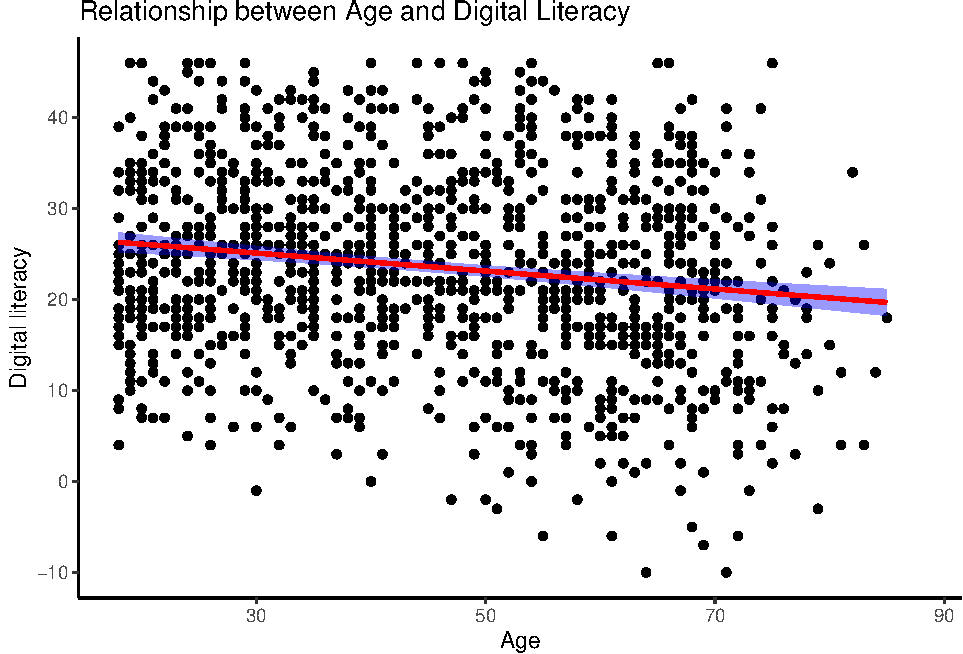
\includegraphics{Replication2019_files/figure-latex/plot1-1.pdf}
To begin with, I examined the relationship between age and digital literacy. The reason is that it is widely assumed that older people tend to have lower digital abilities to access the information resources over the internet. As Figure \label{fig:plot1} \ref{fig:plot1}, there is a negative relationship between age and digital literacy, suggesting that age is a negative predictor of digital literacy. This may explain why older people tend to believe in fake news and misinformation.

\hypertarget{digital-literacy-and-accuracy-discernment}{%
\subsection{Digital Literacy and Accuracy Discernment}\label{digital-literacy-and-accuracy-discernment}}

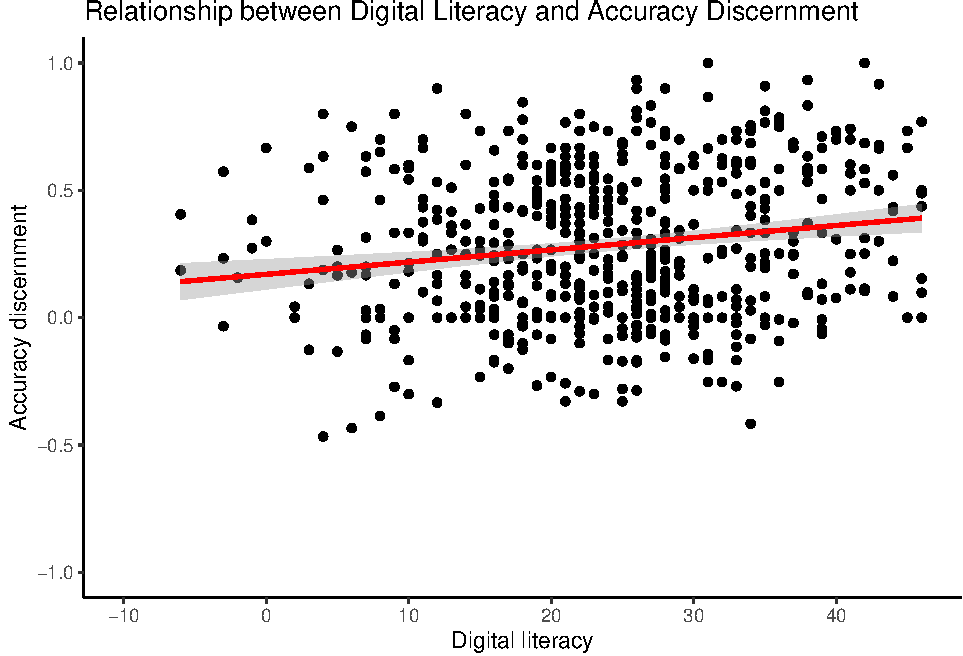
\includegraphics{Replication2019_files/figure-latex/plot2-1.pdf}
Figure \label{fig:plot2} \ref{fig:plot2} shows that digital literacy is positive predictor of accuracy discernment. More digitally literate individuals are more likely to show higher accuracy discernment in misinformation. Therefore, digital literacy translates into higher sharing discernment.

\hypertarget{digital-literacy-and-sharing-discernment}{%
\subsection{Digital Literacy and Sharing Discernment}\label{digital-literacy-and-sharing-discernment}}

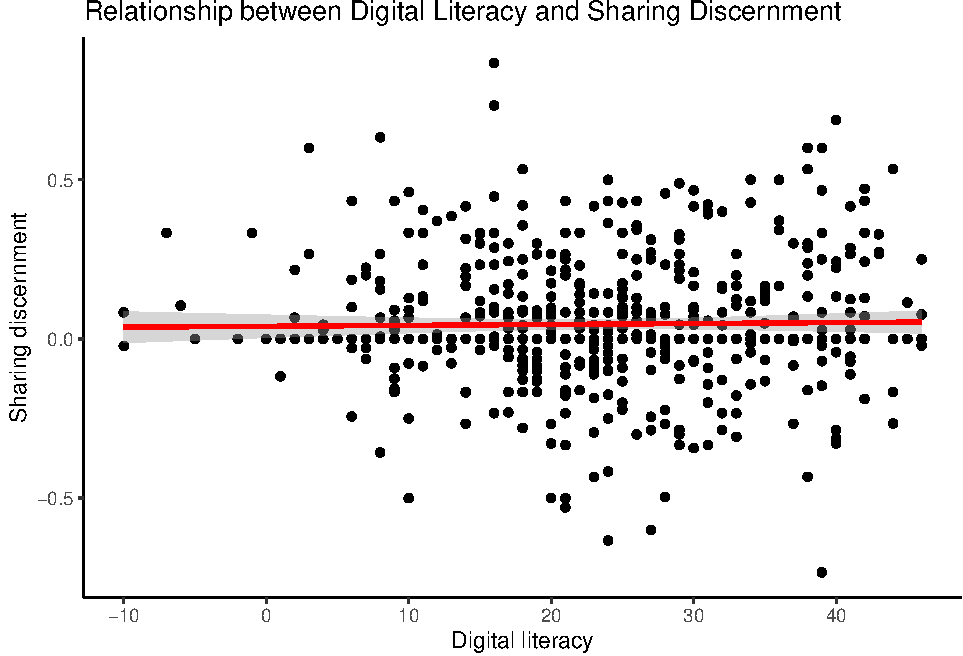
\includegraphics{Replication2019_files/figure-latex/plot3-1.pdf}

Figure \label{fig:plot3} \ref{fig:plot3} shows that digital literacy measure is not associated with sharing discernment. The tendency for individuals to share true news is not more than false news, in other words, sharing intention is not significantly associated with the veracity of news headlines.

\hypertarget{new-knowledge-and-accuracy-discernment}{%
\subsection{New Knowledge and Accuracy Discernment}\label{new-knowledge-and-accuracy-discernment}}

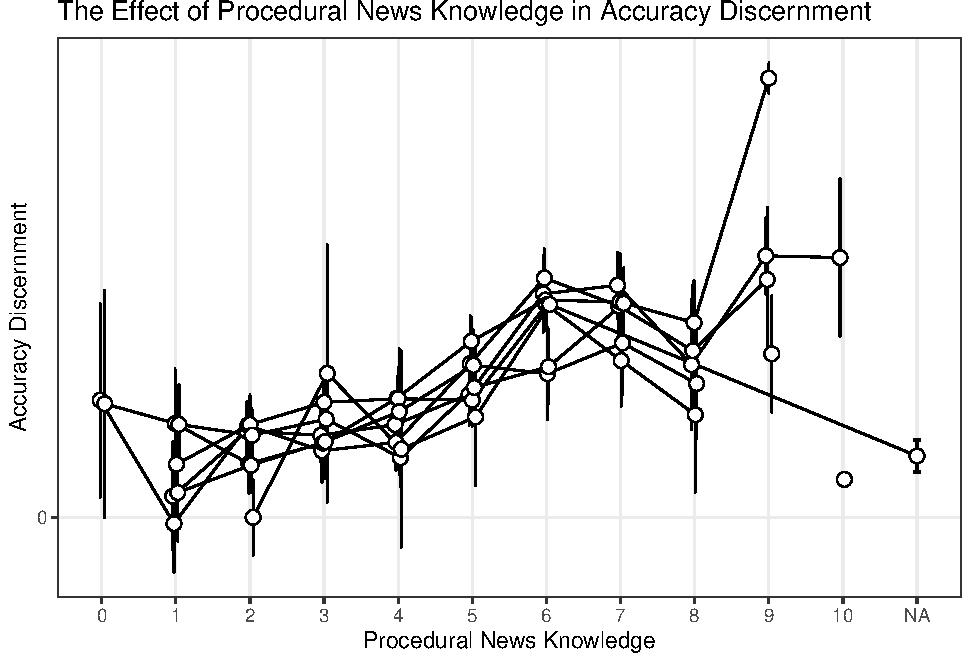
\includegraphics{Replication2019_files/figure-latex/plot4-1.pdf}
Figure \label{fig:plot4} \ref{fig:plot4} shows the relationship between new knowledge and accuracy discernment in misinformation. In general, higher levels of news knowledge lead to higher level of accuracy discernment in misinformation.

\hypertarget{cognitive-reflection-and-digital-literacy}{%
\subsection{Cognitive Reflection and Digital Literacy}\label{cognitive-reflection-and-digital-literacy}}

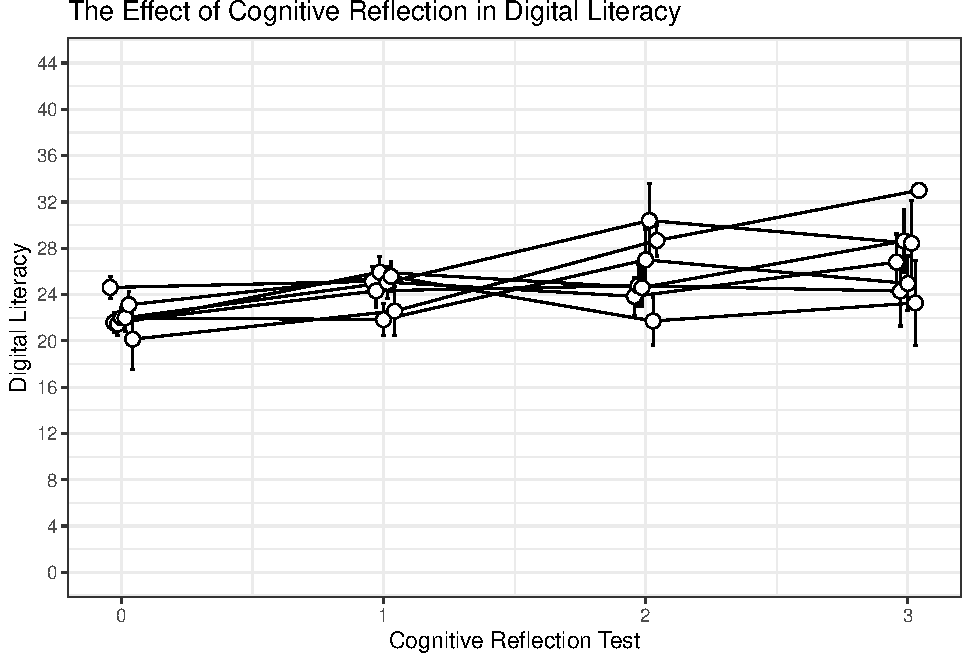
\includegraphics{Replication2019_files/figure-latex/plot5-1.pdf}

Figure \label{fig:plot5} \ref{fig:plot5} shows the relationship between Cognitive Reflection Test and igital Literacy. It appears that higher cognitive reflection test score slightly leads to higher digital literacy skills. However, the relationship is not significant.

\hypertarget{results}{%
\section{Results}\label{results}}

\hypertarget{model}{%
\subsection{Model}\label{model}}

A linear regression model is specified as follows to describe the relationship between dependent and independent variables.

\[
\ Y_i = \beta_0+ \beta_{i} X_{i}+ \epsilon_i
\]

where \(Y_i\) refers to accuracy discernment or sharing discernment in misinformation; while \(\beta_i\) refers to independent variables, including Cognitive Reflection Test Score, Procedural News Knowledge, Self-report Internet Familiarity (Digital Literacy), Education, Age, Gender, Race, Political Ideology.

\begin{table}[!htbp] \centering 
  \caption{Regression Models} 
  \label{} 
\small 
\begin{tabular}{@{\extracolsep{1pt}}lcc} 
\\[-1.8ex]\hline 
\hline \\[-1.8ex] 
 & \multicolumn{2}{c}{\textit{Dependent variable:}} \\ 
\cline{2-3} 
 & Accuracy Discernment & Sharing Discernment \\ 
\hline \\[-1.8ex] 
 Cognitive Reflection Test & 0.04$^{***}$ & $-$0.01 \\ 
  & (0.02, 0.07) & ($-$0.03, 0.01) \\ 
  & & \\ 
 Procedural News Knowledge & 0.03$^{***}$ & 0.01 \\ 
  & (0.02, 0.05) & ($-$0.003, 0.01) \\ 
  & & \\ 
 Digital Literacy & 0.01$^{***}$ & 0.001 \\ 
  & (0.003, 0.01) & ($-$0.0003, 0.003) \\ 
  & & \\ 
 Education & $-$0.04$^{*}$ & 0.01 \\ 
  & ($-$0.09, 0.002) & ($-$0.02, 0.04) \\ 
  & & \\ 
 Age & 0.002$^{***}$ & 0.002$^{***}$ \\ 
  & (0.001, 0.004) & (0.001, 0.003) \\ 
  & & \\ 
 Gender & 0.06$^{***}$ & 0.02 \\ 
  & (0.01, 0.10) & ($-$0.01, 0.06) \\ 
  & & \\ 
 Race & 0.002 & $-$0.004 \\ 
  & ($-$0.05, 0.05) & ($-$0.04, 0.03) \\ 
  & & \\ 
 Ideology & $-$0.13$^{***}$ & $-$0.04$^{**}$ \\ 
  & ($-$0.18, $-$0.08) & ($-$0.08, $-$0.01) \\ 
  & & \\ 
 Constant & $-$0.09$^{*}$ & $-$0.06 \\ 
  & ($-$0.19, 0.01) & ($-$0.13, 0.02) \\ 
  & & \\ 
\hline \\[-1.8ex] 
R$^{2}$ & 0.24 & 0.05 \\ 
F Statistic & 22.98$^{***}$ (df = 8; 582) & 3.89$^{***}$ (df = 8; 622) \\ 
\hline 
\hline \\[-1.8ex] 
\textit{Note:}  & \multicolumn{2}{l}{$^{*}$p$<$0.1; $^{**}$p$<$0.05; $^{***}$p$<$0.01} \\ 
 & \multicolumn{2}{l}{The table reports coefficients, p values, and confidence intervals} \\ 
\end{tabular} 
\end{table}

Table \label{tab:table} \ref{tab:table} shows the regression results for both models. In the regression model where accuracy discernment is the dependent variable, the variables of Cognitive Reflection Test, Procedural News Knowledge, Age, Gender, Ideology are statistically significant at the level of .01, suggesting that the model itself is robust in predicting accuracy discernment in misinformation.
The other model, which examines the relationship between sharing discernment and other variables, shows that Age and Ideology are two critical variables to predict sharing discernment. Age is positively associated with sharing behaviors (p\textless.01); political ideology is negatively associated with sharing behaviors, which suggests that the more liberal an individual is, the less likely he or she shares misinformation (l\textless{} .05).

\hypertarget{discussion-and-conclusion}{%
\section{Discussion and conclusion}\label{discussion-and-conclusion}}

Overall the replication lends empirical support to the original study. The ``Accuracy Discernment'' model well predicts participants' ability to discern authentic headlines from false headlines, holding other variables constant. Digital literacy is positively associated with the increase of truth discernment, which suggests that increasing digital education could potentially increase social media users' ability to recognize accurate information. Additionally, the research results also show that age is negatively associated with digital literacy. THis implies that older people may face more information obstacles to access quality information, therefore, they are more likely to fall far misinformation. News knowledge is also positively associated with digital literacy, suggesting that the more news knowledge an individual gains, the more likely he or she has higher levels of digital knowledge and hence is better at discerning truth from falsehoods.

The results also show that digital literacy does not predict sharing discernment. This finding is consistent with the original study. The ``Sharing Discernment'' model provides support for this finding as only age and political ideology are associated with sharing behaviors, while digital literacy is not a factor predicting misinformation sharing behaviors.

\newpage

\hypertarget{references}{%
\section*{References}\label{references}}
\addcontentsline{toc}{section}{References}

\hypertarget{refs}{}
\begin{CSLReferences}{1}{0}
\leavevmode\hypertarget{ref-r}{}%
R Core Team. 2013. \emph{R: A Language and Environment for Statistical Computing}. Vienna, Austria: R Foundation for Statistical Computing. \url{http://www.R-project.org/}.

\leavevmode\hypertarget{ref-sirlin2021digital}{}%
Sirlin, Nathaniel, Ziv Epstein, Antonio A Arechar, and David G Rand. 2021. {``Digital Literacy Is Associated with More Discerning Accuracy Judgments but Not Sharing Intentions.''} \emph{Harvard Kennedy School Misinformation Review}.

\end{CSLReferences}

\end{document}
